% ==============================================================================
% Tese - Marcos Alécio Spalenza
% Capítulo 2 - Revisão da Literatura
% ==============================================================================
\chapter{Revisão da Literatura}
\label{cap-literatura}


A classificação de documentos, tradicional área de ML, pode ser subdividida segundo sua motivação ou o conteúdo do conjunto de documentos. A classificação de documentos envolve treinar algoritmos de classificação com exemplos rotulados para replicar métodos de identificação de conteúdo e rotulação feitos por um especialista \cite{baeza2011}. Cada conjunto de documentos podem ser chamados também como \textit{dataset}, base de dados ou \textit{corpus}. A coleção destes, porém, é denominada \textit{corpora}. Portanto, para além da origem e conteúdo dos documentos, o algoritmo deve se adaptar para especialização na triagem dos documentos de acordo com suas características.

O especilista realiza uma leitura dos documentos e identifica informações específicas que justificam a categoria atribuída. Para replicar tal tarefa, através da análise do conteúdo, o sistema deve identificar características que estão diretamente relacionadas com a classe que será atribuida. Dependendo da característica dos documentos, o conteúdo relevante pode incluir a identificação de poucas palavras-chave até a formação de modelos linguísticos complexos \cite{jurafsky2009}. Isso acontece também com os SAG, aplicando análises complexas da relação textual para atribuição de notas \cite{paiva2012, yang2021}.

Deste modo, a atribuição de notas torna os SAG uma complexa tarefa de classificação de documentos. Para um modelo SAG é essencial a adaptação do algoritmo de acordo com o método de classificação utilizado pelo especialista. A subjetividade do critério de avaliação deve ser levada em consideração apesar do conteúdo textual \cite{pado2021}. A combinação entre o reconhecimento do modelo avaliativo e do modelo textual deve atender às expectativas do professor na avaliação \cite{condor2020}. Enquanto em parte das atividades as notas podem ser fortemente correlacionadas com a ocorrência dos termos, em outras o critério pode ter alto nível de subjetividade \cite{azad2020}. Então, para a construção de um SAG, são aspectos determinantes a análise contextual das respostas e a compreensão do formato avaliativo do professor \cite{mohler2011}.

\section{\textit{Computer-Assited Assessment}}

A sala de aula é um ambiente rico em conteúdo. As informações produzidas são descritores para o desempenho dos estudantes em sala. A análise desses dados é essencial para o acompanhar o aprendizado dos alunos, verificar a necessidade de reforço do conteúdo e monitorar o cumprimento do curricular \cite{sweta2021}. Tradicionalmente essa dinâmica faz parte dos métodos de ensino-aprendizagem empregados pelos professores, porém, superam a capacidade analítica dos mesmos \cite{madero2019}. Por conta disso, ganharam maior notoriedade e espaço prático os sistemas de EDM, amplificando a análise dos materiais produzidos em sala \cite{siemens2012, romero2010}.

Em EDM, a aquisição de conhecimento aplicado a dados educacionais visa o apoio ao tutor e acompanhamento do ensino \cite{ferreira-mello2019}. A consequência da mineração de dados nesse cenário é uma expressiva redução da carga horária do professor voltada para o acompanhamento coletivo e individual \cite{sweta2021}. Essa redução ocorre com o professor passando para papeis de monitoramento e auditoria dos resultados.

Portanto, através da mineração de dados, é possível a análise de todo material produzido pelos alunos, a criação de \textit{feedbacks} individuais e a aplicação de reforço para determinados grupos de estudantes. Os SAG, uma das áreas de estudo em EDM, estão diretamente associados com essas três características \cite{burrows2015}. Os SAG são responsáveis pela avaliação em massa de respostas textuais curtas, replicando o critério avaliativo do professor. Os SAG fazem parte de um grupo de técnicas computacionais para apoio aos métodos avaliativos, conhecidos pelos estudos em CAA \cite{perez-marin2009}.

A verificação do aprendizado nas questões discursivas curtas contribuem para identificar se os estudantes assimilaram ou não o conteúdo ministrado em sala \cite{oliveira2013}. Além disso, a aplicação deste tipo de atividade é base para prática da escrita, busca de informações e sumarização de conteúdo. Portanto, tais atividades realizam uma função importante para todos os níveis de ensino, principalmente durante o desenvolvimento da escrita \cite{johnstone2002}. 

Com a alta carga-horária do professor, existe baixo índice de aplicação desse tipo de questão dada sua relavância \cite{bilgin2017}. Assim, considerando o tempo em sala, os esforços de o planejamento, revisão e análise das atividades acabam sendo tratados como secundários. O apoio computacional nesta tarefa reduz o tempo que é necessário para avaliação do conteúdo fora de sala de aula, com o professor participando parcialmente da atribuição de notas \cite{ming2005}. Neste processo, os sistemas replicam o critério avaliativo do professor, com este garantindo a coerência da avaliação, fazendo o sistema seguir fielmente seu critério. Adicionalmente, as aplicações de ML nesse cenário, refletem em modelos descritivos de correção, formando \textit{feedbacks} aplicados diretamente em sala de aula \cite{butcher2010, bernius2022}. 

No entanto, para interpretação computacional, as questões devem ser elaboradas com objetividade \cite{bailey2008}. Nesse aspecto, dentro de um tema, deve ser possível identificar alinhamento entre as respostas, definindo se cada uma segue ou não o que compõe o critério avaliativo. Assim, as questões discursivas \cite{bezerra2008} envolvem a liberdade de escrita dos estudantes na formulação das respostas. A Figura \ref{fig-atividades} caracteriza as formas de atividades segundo seu modelo de resposta \cite{spalenza2017}.

\begin{figure}[!h]
\centering
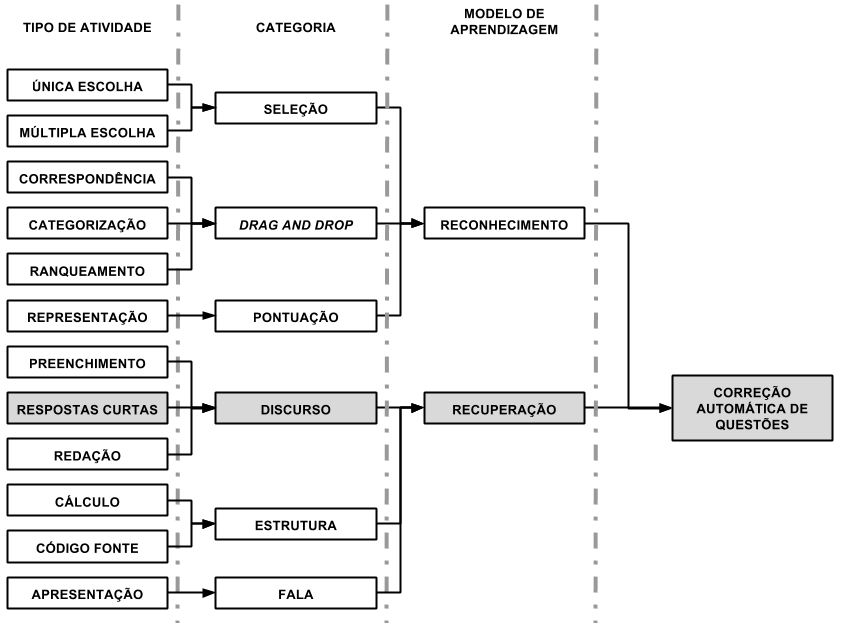
\includegraphics[width=\textwidth]{figuras/tiposAtividade}
\caption{A extração da informação e os tipos tradicionais de atividade aplicadas no cotidiano de sala de aula.}
\label{fig-atividades}
\end{figure}

Como apresentado na Figura \ref{fig-atividades} o professor dispõe de alguns modelos de atividades que, refletem diferentes aspectos do aprendizado. Temos quesões que são abertas e com pouca ou nenhuma restrição como as redações \cite{almeida-junior2017} ou respostas fechadas para uma única palavra, guiadas pelo enunciado. As respostas discursivas encontram-se em âmbito intermediário \cite{bailey2008}. As respostas curtas, por sua essência, visam estabelecer a relação entre o conhecimento do aluno e o conteúdo encontrado no material didático. A Figura \ref{fig-SAG-concepts} demonstra como o espectro de questões trabalhados através das respostas discursivas curtas \cite{spalenza2017}.

\begin{figure}[!h]
\centering
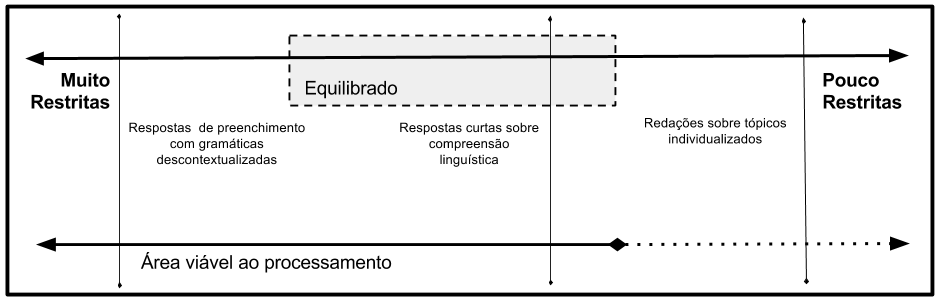
\includegraphics[width=\textwidth]{figuras/aprendizadoSAG}
\caption{Extração de informação em questões discursivas: entre respostas pequenas não-convergentes e a subjetividade das competências na avaliação de redações.}
\label{fig-SAG-concepts}
\end{figure}

A Figura \ref{fig-SAG-concepts} posiciona as respostas curtas enquanto um nicho das questões discursivas. O ideal é que, dentre os conhecimentos, a questão deve evitar abordar temas de cunho interpretativo ou temas individuais, que tangenciam experiências específicas de cada aluno \cite{siddiqi2008}. A representação da resposta deve ser completa, com a resposta dando embasamento para a correção, evitando informações restritas ou codificadas \cite{ding2020}. O enunciado deve guiar o aluno, de forma que as respostas sejam convergentes \cite{suzen2020, filighera2020}. Para isso, é fundamental que o sistema realize ao menos três etapas. A primeira etapa é o aprendizado do modelo de respostas do aluno \cite{ramachandran2015b}. A segunda etapa é reconhecer o padrão avaliativo do professor através do modelo de respostas \cite{funayama2020}. A terceira etapa é replicar o modelo avaliativo e elaborar \textit{feedbacks} coerentes \cite{fowler2021}.


\section{\textit{Active Learning}}

Em ML, o aprendizado ocorre com a formação de conhecimentos a partir da interpretação dos padrões \cite{bishop2006}. Esse procedimento dita a forma de aquisição de conhecimento do sistema para treinamento de modelos, buscando desempenho similar ao humano. Neste trabalho apresentamos um método de amostragem por \textit{Active Learning} \cite{miller2020, kumar2020}, com anotação iterativa do professor em itens selecionados através das etapas de clusterização \cite{horbach2018}. Presente uma série de sistemas SAG, as técnicas de clusterização utilizam \textit{Unsupervised Learning} para avaliação com base na similaridade das amostras \cite{basu2013, zhang2016, marvaniya2018}. Porém, os trabalhos na literatura geralmente utilizam \textit{Supervised Learning}, criando modelos através de uma série de amostras pré-avaliadas pelo especialista.

Portanto, a grande maioria dos estudos utiliza o particionamento entre treino e teste dos dados, de acordo com o determinado em cada \textit{dataset}. Considerando cada resposta dos estudantes uma amostra, o particionamento em treino e teste reflete a divisão \textit{a priori} do conjunto de dados em um grupo para criação do modelo e outro para avaliação \cite{heilman2015}. Esse formato clássico permite ao sistema observar apenas uma parcela dos dados para reconhecimento dos padrões, realizando a inferência nas demais amostras até o momento desconhecidas \cite{bishop2006}. Assim, esses sistemas utilizam um conjunto de treino para extração do critério avaliativo, criando o modelo para replicar o método de atribuição de notas, pressupondo a equivalência dos mesmos.

O conjunto de amostras de treino e teste não tem necessariamente a mesma origem \cite{sung2019a}. O uso dos sistemas SAG pelo professor compreende sua aplicação durante a disciplina. Portanto, uma atividade avaliada com um modelo SAG pode ser utilizada para uma série de aplicações, em um diferente momento e com outro grupo de estudantes. Com uma nova iteração, outros tópicos podem ser levantados em cada resposta. A tendência nesses casos é a avaliação incorreta de parte dos dados por conta da rigidez do conjunto fixado para o treinamento.

Alguns métodos também são baseados em exemplos da resposta-alvo, denominadas respostas candidatas \cite{banjade2015, roy2016}. As respostas candidatas, são amostras elaboradas pelo professor e anotadas para representar seus padrões avaliativos. Os sistemas SAG com base nesse tipo de dado buscam, em geral, a comparação direta entre as respostas e o índice de sobreposição \cite{jimenez2013, kar2017, zhang2020}. Porém, as limitações dos dados em análise são um contraponto à liberdade textual das questões discursivas curtas. Este tipo de treinamento gera uma tendência na avaliação, com limitações na capacidade do modelo interpretar conteúdos adversos nas respostas dos alunos \cite{ramachandran2015a}. Além de tornar-se engessada, a resposta candidata também não garante o alinhamento para os demais documentos do \textit{dataset}.

Dentro desse contexto, para contornar parcialmente as limitações, ainda existem alguns métodos que utilizam mais informações sobre a atividade na etapa de treinamento, como o enunciado, o material de apoio e o quadro de \textit{rubrics}\cite{ramachandran2015b, wang2019}. O enunciado e o material de apoio adicionam ao sistema conhecimento externo sobre o tema. Enquanto as respostas candidatas e o quadro de \textit{rubrics} são materiais descritivos do modelo avaliativo do professor para todos, inclusive o próprio SAG \cite{mizumoto2019, marvaniya2018}. Existem ainda sistemas que precisam de mais detalhes sobre a avaliação, com a confecção de regras e filtros de conteúdo \cite{butcher2010, pribadi2017}.

Para lidar com a diversidade textual também são empregadas estratégias de \textit{Data Augmentation}. Com \textit{Data Augmentation} as amostras passadas como treinamento são combinadas para representar de forma mais complexa o modelo avaliativo. O uso do aumento de dados torna os sistemas tradicionais um pouco mais robustos a alterações e mudanças nos padrões básicos, reduzindo a ocorrência de classificações tendenciosas \cite{kumar2019, lun2020}. Assim, a quantidade de amostras para treinamento e variações para cada modelo de resposta torna-se muito superior à quantidade dada inicialmente.

Diferente das técnicas citadas, o método proposto de \textit{Active Learning} prioriza a seleção das principais amostras para otimização do esforço de anotação \cite{kumar2020}. A proposta combina os métodos de \textit{clusterização} \cite{spalenza2019} e classificação \cite{oliveira2014} para identificação iterativa dos diferentes tópicos abordados nas respostas. Assim, a evolução do conjunto de dados acontece durante cada uma das iterações. A clusterização, via \textit{Unsupervised Learning}, não recebe dados anotados e extrai as respostas distintas com base no nível de similaridade \cite{everitt2011}. E a classificação, via \textit{Supervised Learning}, coleta as anotações do especialista nas amostras selecionadas para treinamento do modelo \cite{bishop2006}. A partir daí que o modelo treinado replica a avaliação para as demais respostas.


\section{Processamento de Linguagem Natural}

Para criação de um modelo linguístico, os sistemas utilizam técnicas de NLP como estratégias de aquisição de informação. As primeiras técnicas de SAG da literatura e os primeiros sistemas propostos utilizavam descritores \cite{galhardi2018a}. Os descritores são caracteríticas simples extraídas segundo o formato da escrita de cada documento. Em geral, são formados por características pré-definidas, de acordo com a estrutura da resposta do aluno, sem levar em consideração a profundidade do conteúdo \cite{mohler2009}. Dentre os descritores, os mais comuns eram a contagem de erros da linguagem, a quantidade de palavras e a frequência de certas classes gramaticais \cite{ galhardi2018b, riordan2019}. Porém, tais características pré-definidas não atendem a uma grande quantidade de respostas, criando modelos linguísticos com pouca aderência ao conteúdo.

Posteriormente, surgiram estruturas para maior aquisição de informação e modelagem linguística ao observar os diferentes propósitos das questões discursivas curtas e sua aplicação multidiciplinar \cite{saha2018, kumar2019}. Nesse novo cenário, os modelos linguísticos ampliaram a aderência do sistema ao tema das atividades. Através do conjunto de respostas, os sistemas começaram a elaborar modelos linguísticos contextuais, até o momento suficientes para encontrar associações entre as palavras \cite{tan2020}. A partir dessas associações, os sistemas estabeleceram as primeiras conexões entre os termos de cada respostas e o critério avaliativo do professor \cite{sahu2020}.

A evolução das estratégias, agora voltadas para análise do texto por completo, adicionaram mais informações aos SAG. Porém, a resposta é dada por detalhes do conjunto de respostas, sendo o todo não necessariamente relevante para avaliação. Nesse aspecto, podemos citar como adições importantes as técnicas de seleção de características, ponderação e reconhecimento de padrões \cite{banjade2016}. Para ponderação textual o modelo mais comum é o Term Frequency - Inverse Document Frequency (TF-IDF) \cite{baeza2011}. O TF-IDF é um método clássico que realiza a ponderação de acordo com a frequência dos termos, equilibrando a relevância de cada termo segundo sua ocorrência nos documentos e no \textit{dataset} \cite{sultan2016}. Entretanto, com a evolução dos métodos neurais, ficaram em evidência as \textit{word embeddings} \cite{jurafsky2009}. As \textit{embeddings} são modelos linguísticos de grande dimensionalidade adquiridos de uma coleção de documentos \cite{goldberg2017}. Esses modelos analisam a conexão semântica dado o emprego conjunto dos pares de termos em \textit{corpora} de larga escala. Assim, de forma pareada, os sistemas avaliam o nível de correspondência dos termos pelo contexto. A partir disso, os sistemas SAG avaliam a proximidade entre as respostas dos estudantes para diferentes termos, frases e contextos \cite{sung2019b, ghavidel2020, galhardi2020, haller2022}.

Por outro lado, na seleção de características e sumarizalção de conteúdo, se destacaram as técnicas como o \textit{Latent Semantic Analysis} (LSA) \cite{landauer1998}, \textit{Latent Dirichlet Allocation} (LDA) \cite{blei2003}. O LSA é uma das mais utilizadas na literatura \cite{basu2013, sahu2020}. O uso desta técnica compreende identificar relações semânticas dentro do conjunto de respostas \cite{mohler2009}. Assim, através do LSA, os sistemas reunem o conteúdo que potencialmente contém maior significância no tema. O mesmo intúito é compartilhado pelo LDA. Esse algoritmo utiliza a análise probabilística para \textit{ranqueamento} dos termos encontrados no texto segundo sua identificação com grupos de documentos. No âmbito dos SAG, essa técnica de extração de tópicos, é utilizada para agrupamento pelas referências encontradas em cada grupo de nota \cite{basu2013, zhang2022}.

Entretanto, nesse nível, os modelos os modelos linguísticos criados através da frequência dos termos de cada resposta dos estudantes ainda não refletem uma análise complexa tal qual a do especialista. Portanto, na literatura existem estudos que propõe maior extração de informação textual, ainda que em textos curtos, para formação de componentes linguísticos mais robustos \cite{saha2018, zesch2018}. Assim, foram realizadas análises da estrutura textual segundo suas camadas de construção, sejam elas sintática, semântica, léxica, morfológica ou gramatical \cite{ramachandran2015b, roy2016}. Ainda nessa linha, alguns estudos também remontam o contéudo das respostas sob a perspectiva sequencial da construção textual \cite{kumar2017}. Essas sequências subdividem cada resposta em pequenos trechos que contém de 1 a \textit{n} termos para aplicar na análise de equivalência e sobreposição entre respostas \cite{jimenez2013, sakaguchi2015, sultan2016}.

Os modelos de DL também contribuiram nessa linha. Utilizando técnicas de \textit{Continuous Bag-of-Words} (CBoW) ou \textit{skip-gram} e suas derivações, estes construiram representações de padrões mais complexos da vizinhança dos \textit{tokens} \cite{mikolov2013}. Essas técnicas buscam a identificação contextual em segmentos do conteúdo com a atribuição de pesos ponderando sua relevância. Assim, as redes neurais substituiram boa parte das estratégias de quantificação de equivalência e a aplicação das métricas de sobreposição \cite{haller2022}. Através das redes, foram incorporadas melhores formas de identificar a ocorrência dos segmentos de termos. Com tais segmentos, são aplicadas enriquecimentos estruturais e semânticos na análise documental \cite{camus2020}. No entanto, uma dificuldade encontrada na construção destes SAG são os \textit{datasets} com poucas amostras para treinamento \cite{bonthu2021}. Com o avanço dos SAG, a combinação dos aspectos de NLP que investigam a forma e construção de cada sentença devem contemplar também tais representações de vizinhança das respostas \cite{riordan2019, kumar2019}.


\section{Avaliadores de Questões Discursivas Curtas}

Os sistemas SAG, para uma análise documental complexa, são compostos por um conjunto de métodos que incluem a criação do modelo linguístico, organização do conhecimento e a identificação de características relevantes. Apesar disso, uma parte fundamental dos sistemas SAG são os classificadores de alta qualidade \cite{funayama2020}. Portanto, são os classificadores que destacam o conhecimento adquirido nas etapas anteriores e o apredizado do modelo avaliativo \cite{mohler2011}.

O propósito do classificador é compreender, replicar e descrever o modelo do professor (especialista) \cite{yang2021}. Assim, é função do sistema identificar caracerísticas relevantes para assimilar a forma que o professor avalia cada resposta enviada pelos estudantes \cite{jordan2012, mao2018}. Em geral, os avaliadores automáticos são divididos segundo quatro diferentes técnicas: por mapeamento de conceitos, extração de informação, análise de \textit{corpus}, algoritmos de ML \cite{burrows2015}. 

O método de mapeamento de conceitos consiste em um processo de detecção de determinado conteúdo nas respostas produzidas pelos estudantes. O reconhecimento de conteúdo, portanto, é realizado com análise de alinhamento entre termos de respostas \cite{jimenez2013, zhang2020}. Neste método avaliativo, a principal característica é a existência dos conceitos nas respostas de maior grau de nota \cite{kar2017, chakraborty2017}. Porém, mesmo com a construção automática de padrões através da amostragem, não é garantida a consistência dos modelos produzidos \cite{azad2020}. Deste modo, tendo como principal fator a compatibilidade entre respostas, o mapeamento de conceitos tende a ser muito dependente do objetivo da questão e do conteúdo do conjunto de respostas \cite{filighera2020}.

Já a extração de informação, apresenta sistemas caracterizados por um primeiro contato com estratégias de identificação factual e contextual. Nestes modelos, existe uma evolução dos métodos para análise do conteúdo, sendo compostos por técnicas de reconhecimento de padrões e séries de expressões regulares \cite{ramachandran2015b, butcher2010}. Assim, sistemas SAG com base na extração de informação apresentam uma coleção de padrões em análise para o alinhamento entre a resposta e a expectativa do professor \cite{tan2020}. Então, o modelo de avaliação utilizado se aproxima da leitura do professor. Porém, até aqui, estas técnicas atendem apenas aos modelos pré-definidos.

Os métodos baseados em \textit{corpus} distinguem-se pelo uso da análise estatística com base na frequência dos termos em cada conjunto de dados \cite{kumar2019}. Neste método, os sistemas utilizam a linguagem para validação do alinhamento entre respostas, interpretar variações de uso e caracterização do conteúdo \cite{ziai2012, menini2019}. Para além dos termos, essas técnicas aplicam adição de informação para maior diversidade semântica, tornando modelos mais flexíveis para análise do vocabulário do material \cite{fowler2021}.

Apesar da consistência dos modelos anteriores, em um âmbito geral existem limitações para aplicação de cada uma das técnicas em diferentes \textit{datasets} \cite{riordan2019, ding2020}. Em geral, as representações do critério avaliativo por parte do especialista por si não representam bem o conhecimento para sua reprodução pela sistema \cite{filighera2020}. Em contraste aos modelos superficiais, as técnicas de ML foram incorporadas na análise textual para criação de modelos mais robustos, com fundamentação estatística \cite{galhardi2018b}. Assim, esses modelos visam compreender o conteúdo dos documentos, pelas diferentes componentes textuais, para realizar o reconhecimento de padrões \cite{suzen2020}. Distintamente das técnicas baseadas em regras e expressões regulares, os modelos de ML são capazes de se adaptar para diferentes temas e modelos de resposta \cite{zhang2016, saha2019, camus2020}. Portanto, a capacidade de adaptação destes modelos permite a associação de padrões não convergentes. Como consequência, mesmo com amostras divergentes, existe a formação de critérios mais complexos para atribuição da nota.

Em geral, um objetivo dos sistemas SAG, descrito pela literatura, é mesclar os métodos e suas dinâmicas de aprendizado para evolução do modelo avaliativo \cite{burrows2015, zesch2018}. Deste modo, é essencial a construção de modelos que reproduzam com alta qualidade a atribuição de notas realizada pelo especialista \cite{jordan2012}. Apesar das dificuldades e dos detalhes subjetivos da avaliação \cite{roy2018}, o intúito é que o desenvolvimento do SAG compreenda a relação entre diferentes características de avaliação e a capacidade de atender diferentes domínios \cite{sung2019a, saha2019}. Nesse contexto, esperamos o desenvolvimento de sistemas mais robustos, que compreendam o vínculo entre o critério avaliativo e a escrita dos estudantes.
